\begin{pastexam}[label={px:gk3-097-ds-03}]{高考三級資訊處理 97 年 第三題}
（申論）

有關圖形與樹的名詞：（每小題 5 分，共 25 分）
\begin{itemize}[leftmargin=2.2em, nosep]
\item[㈠] 請說明何謂擴張樹（Spanning Tree）。
\item[㈡] 請說明何謂雙連通圖（Biconnected Graph）。
\item[㈢] 請說明何謂二分圖（Bipartite Graph）。
\item[㈣] 請說明每個樹是否均屬於二分圖。
\item[㈤] 請說明每一個高度平衡二元樹（AVL）是否均屬於完滿二元樹（Fully Binary Tree）。
\end{itemize}
\end{pastexam}

\begin{pastsoln}
㈠㈡㈢是定義（資結書第~21.1~節、第~23.5~節、第~21.6~節），㈣㈤是判斷題，要給證明或反例。 ㈤屬於
資結書第~7、10~章的內容，因為和㈣一起考「某類樹是不是某類圖或樹」，放在這裡。

\textbf{㈠ 擴張樹。} 設 $G = (V, E)$ 是無向連通圖。 $G$ 的擴張樹（生成樹）是一個子圖
$T = (V, E')$，$E' \subseteq E$，包含 $G$ 的\textbf{全部}頂點，而且 $T$ 本身是一棵樹（連通、沒有環）。
所以 $T$ 恰好有 $|V| - 1$ 條邊。 例如在圖上做 DFS 或 BFS，走訪時用到的邊就構成一棵擴張樹（DFS
樹、BFS 樹）；邊有權重時，權重和最小的擴張樹就是最小生成樹（資結書第~24~章）。 不連通的圖沒有
擴張樹，只有擴張森林。

\textbf{㈡ 雙連通圖。} 無向連通圖 $G$ 裡，若刪掉頂點 $v$（和它的邊）之後圖變成不連通，$v$ 叫做
割點（articulation point）。 \textbf{沒有割點}的連通圖叫雙連通圖。 等價的說法（頂點數至少 $3$ 時）：
任兩個頂點之間至少有兩條除了端點以外不共用頂點的路徑，所以刪掉任何一個頂點，其他頂點仍然互相
連得到。 例如環 $C_4$ 是雙連通的；一條路徑 $a - b - c$ 不是，因為刪掉 $b$ 就斷了。

\textbf{㈢ 二分圖。} 無向圖 $G = (V, E)$ 若能把頂點分成兩個不相交的集合 $V_1$、$V_2$
（$V_1 \cup V_2 = V$），使得每一條邊的兩個端點一個在 $V_1$、一個在 $V_2$（同一集合裡的頂點之間沒
有邊），就叫二分圖。 等價的條件是：$G$ 沒有長度為奇數的環。 判斷的方法是用 BFS 把頂點輪流塗兩
種顏色，看有沒有一條邊兩端同色（資結書第~21.6~節）。

\textbf{㈣ 是，每一棵樹都是二分圖。}

\textbf{證明。} 任選一個頂點 $r$ 當根，令 $d(v)$ 是 $v$ 到 $r$ 的路徑長（樹中兩點之間的路徑唯一）。
取 $V_1 = \{v : d(v) \text{ 為偶數}\}$，$V_2 = \{v : d(v) \text{ 為奇數}\}$。 樹的每一條邊連接一個
節點和它的父節點，兩者的 $d$ 差 $1$，奇偶不同，所以每條邊的兩端一個在 $V_1$、一個在 $V_2$。 這就
是二分圖的定義。 （也可以這樣說：樹沒有環，當然沒有奇數長的環。）
\hfill$\blacksquare$

\textbf{㈤ 不是。} 這裡的「完滿二元樹」不論照哪一種常見的定義，都有 AVL 樹的反例：
\begin{itemize}
\item 若完滿二元樹指高度 $h$ 而節點數恰為 $2^h - 1$ 的樹（每一層都滿）：只有兩個節點的樹（根和
它的左子節點）是 AVL 樹，根的左右子樹高度差 $1$；它的高度是 $2$，滿的話要有 $2^2 - 1 = 3$ 個節點，
它只有 $2$ 個，不完滿。
\item 若指每個節點的子節點數都是 $0$ 或 $2$（full binary tree 的另一種定義）：同一個例子，根只有
一個子節點，也不符合。
\end{itemize}
\begin{center}
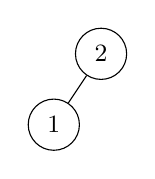
\begin{tikzpicture}[every node/.style={circle,draw,minimum size=6.5mm,inner sep=0pt,font=\small},
  level distance=9mm, sibling distance=12mm]
\node {2} child {node {1}} child[missing];
\end{tikzpicture}
\end{center}
AVL 樹只要求每個節點左右子樹的高度差不超過 $1$（資結書第~10.2~節），允許某些位置缺節點；完滿二
元樹則一個都不能缺。 反過來，照第一種定義，完滿二元樹每個節點的左右子樹一樣高，一定是高度平衡的。
所以完滿二元樹是 AVL 樹的一種，AVL 樹不一定是完滿二元樹。
\end{pastsoln}
